\section{Extraction of Static KG Summaries}
\label{sec:approaches-static}

Static summaries are extracted to reflect the coverage of the original KG. Depending on the application, existing methods cover different targets: data patterns, or query answers.

\subsection{Pattern Coverage-Based Summarization}
\label{sec:approaches-static-pattern}

Entities in KGs are assigned different types, i.e.,~classes, and they are described using different properties. Extracting a summary that exemplifies the most representative data patterns for describing the entities in a KG is an important component of KG profiling~\cite{DBLP:journals/semweb/EllefiBBDDST18}. Existing methods in this category have been focused on extracting summaries that cover data patterns at different granularities, from independent instantiations of classes and properties to their joint instantiations associated with graph structure. Figure~\ref{fig:outline-pattern} outlines the expressivity increases among different data patterns.

\begin{figure}[h]
\centering
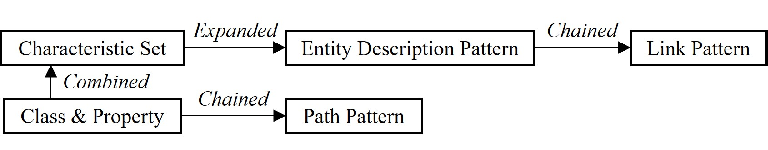
\includegraphics[width=\columnwidth]{figs/outline-pattern.pdf}
\caption{Expressivity increases among data patterns.}
\label{fig:outline-pattern}
\end{figure}

\subsubsection{Class \& Property}
\emph{Class and property} instantiations are the most elementary data patterns in a KG, such as the instances of the class \texttt{Person} and the property \texttt{nationality} in Figure~\ref{fig:example}. To exemplify all such instantiations during KG visualization, the 3-S approach~\cite{DBLP:conf/icde/SundaraAKDWCS10} performs stratified sampling by uniformly sampling the instances of each class and each property independently.
% aggregate entities with the same class, or describing the same entity by a common property. Then entities are sampled from each set to constitute the summary as a directed node-link diagram. For each entity in the summary, its one-hop neighborhood covers all distinct properties describing this entity, where multiple values of each property are aggregated into a single node.
However, this method is only suitable for KGs that have a small schema.

Given a potentially large number of classes and properties used in a KG, the IlluSnip approach~\cite{DBLP:conf/wsdm/ChengJDXQ17} extracts a size-bounded connected subgraph that contains the most frequently instantiated classes and properties, as well as entities having the highest PageRank scores, to illustrate the main content of the KG. For example, the summary in Figure~\ref{fig:illusnip} includes \texttt{Person} and \texttt{act\_in} which are the most frequently instantiated class and property in Figure~\ref{fig:example}, respectively. To fulfill this, a \emph{Maximum-weight-and-coverage Connected Graph} problem (MwcCG) is formulated, and is solved by a greedy approximation algorithm for this new NP-hard optimization problem, where coverage and weights are jointly maximized to account for class/property instantiations and entity scores, respectively.

\begin{figure}[h]
\centering
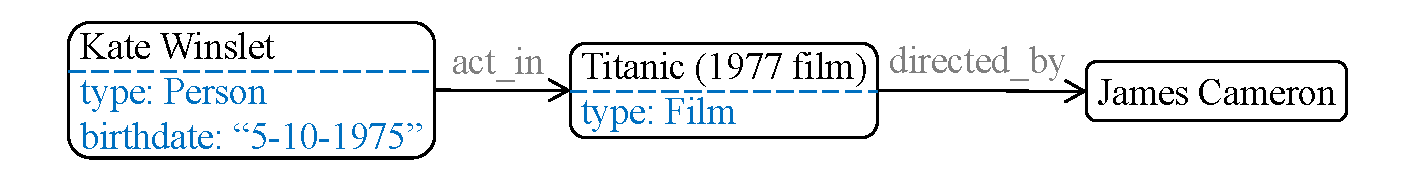
\includegraphics[width=\columnwidth]{figs/illusnip.pdf}
\caption{A summary extracted from Figure~\ref{fig:example} containing the most frequently instantiated class \texttt{Person} and property \texttt{act\_in}.}
\label{fig:illusnip}
\end{figure}

As a follow-up effort, Liu et al.~\shortcite{DBLP:journals/tweb/LiuCLQ19} design more efficient algorithms for MwcCG and adapt them to SPARQL endpoints for summarizing remotely accessed KGs.
% Besides, they also propose an anytime version of the algorithm that can gradually obtain empirically better solutions with extra time.

\subsubsection{Characteristic Set}
On top of individual properties, the \emph{characteristic set}~\cite{DBLP:conf/esws/HelingA20} of an entity is the set of all properties (including \texttt{type}) describing that entity in a KG, and each property can be associated with its average frequency of occurrence among all the entities having this characteristic set. For example, the characteristic set of \texttt{James Cameron} in Figure~\ref{fig:example} consists of $\{$\texttt{nationality}, \texttt{type}$\}$. All the characteristic sets instantiated in a KG, the number of entities having each characteristic set, and the average frequency of each property constitute a statistical profile of the KG which is required by a query optimizer for devising efficient query plans. When it is difficult to access or process the entire KG, Heling et al.~\shortcite{DBLP:conf/esws/HelingA20,DBLP:journals/semweb/HelingA23} use estimations for this profile derived from a KG summary containing the properties of a set of selected entities. Entities that have high outdegrees (i.e.,~rich descriptions) have a high chance of being selected.
% To achieve the estimation, a summary of the KG is extracted as a subgraph induced by a set of sampled entities, which ideally should cover similar proportion of characteristic sets to the original KG, thus maximizing the closeness of profiles computed from the summary and the original KG. Specifically, a set of entities is firstly sampled with equal or biased probability that favors entities with higher outdegree.

\subsubsection{Entity Description Pattern}
In addition to the properties (i.e.,~outgoing edges) in a characteristic set, the \emph{Entity Description Pattern} (EDP)~\cite{DBLP:conf/semweb/00010LXPKQ21} of an entity distinguishes its types from other properties and, further, includes the properties that have this entity as a value (i.e.,~incoming edges).
% Formally, the EDP of an entity is a three-tuple~$\langle C, P_O, P_I \rangle$, where~$C$ is the set of classes assigned to this entity, $P_O$~is the set of properties describing this entity, and~$P_I$ is the set of properties having this entity as value.
For example, Figure~\ref{fig:edp-lp} shows~$E_1$, the EDP of two entities \texttt{Kate Winslet} and \texttt{Leonardo DiCaprio} in Figure~\ref{fig:example}, and~$E_2$, the EDP of \texttt{Titanic (1977 film)} and \texttt{Avatar: The Way of Water}.
% An extractive KG summary that covers popular EDPs not only provides example entities but also exemplifies representative sub-structures of the KG, thus helping the user better understand its content.
To extract a summary of a KG to exemplify all or the most frequent EDPs, the two-step PCSG approach~\cite{DBLP:conf/semweb/00010LXPKQ21}, in its first step, selects the minimum number of connected components that collectively cover those EDPs by formulating and solving a \emph{Set Cover} problem. In the second step, it extracts an optimal subgraph from each selected connected component and merges these subgraphs. Specifically, the subgraph is a tree found by solving a minimum-size \emph{Group Steiner Tree} problem~\cite{DBLP:conf/wg/Ihler91} where all the entities having the same EDP form a group. The extracted minimal tree is required to cover all the groups, i.e., contain at least one entity for each EDP; the types and properties of this entity are then extracted to exemplify its EDP.

\begin{figure}[h]
\centering
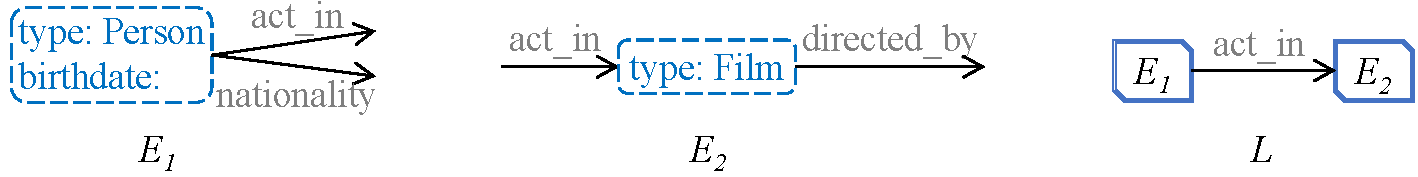
\includegraphics[width=\columnwidth]{figs/edp-lp.pdf}
\caption{Two EDPs ($E_1, E_2$) and a LP ($L$) in Figure~\ref{fig:example}.}
\label{fig:edp-lp}
\end{figure}

\subsubsection{Link Pattern}
Building on EDPs, \emph{Link Pattern} (LP)~\cite{DBLP:conf/semweb/00010LXPKQ21} takes a further step to characterize not only the neighborhood pattern of each individual entity, but also the patterns of relations between entities. Specifically, the LP of a relation between two entities is a triple consisting of the relation type and the EDPs of the two entities. For example, Figure~\ref{fig:edp-lp} shows a LP shared by the three \texttt{act\_in} relations in Figure~\ref{fig:example}.
% Formally, a LP is a three-tuple~$\langle E_O, p, E_I \rangle$, where~$p$ is a property describing an entity~$e_O$ with an entity~$e_I$ as value, while~$E_O$ and~$E_I$ are the EDPs of~$e_O$ and~$e_I$, respectively.
To extract a KG summary that also exemplifies all or the most frequent LPs, the aforementioned PCSG approach~\cite{DBLP:conf/semweb/00010LXPKQ21} extends the formulation of the Group Steiner Tree problem by performing edge subdivision to convert each relation into a node; all the relations having the same LP form a group to be covered by the extracted minimal tree. For example, the summary in Figure~\ref{fig:pcsg} exemplifies the two EDPs and the LP in Figure~\ref{fig:edp-lp}. Note that the EDPs of the entities \texttt{James Cameron} and \texttt{UK} are not fully exemplified in this summary.

\begin{figure}[h]
\centering
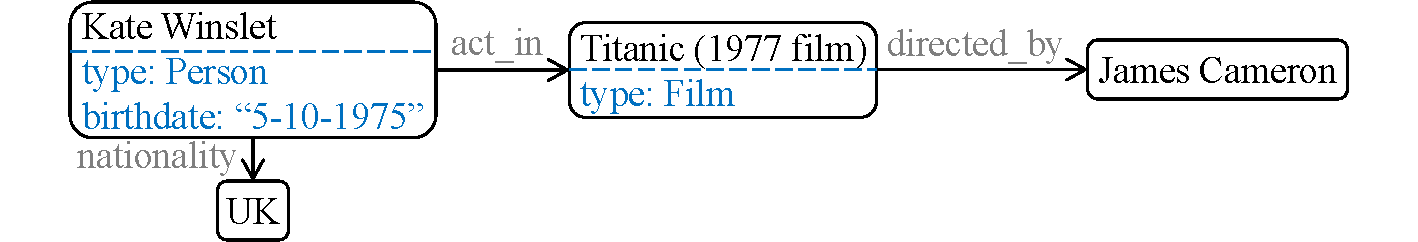
\includegraphics[width=\columnwidth]{figs/pcsg.pdf}
\caption{A summary extracted from Figure~\ref{fig:example} exemplifying the two EDPs and the LP in Figure~\ref{fig:edp-lp}.}
\label{fig:pcsg}
\end{figure}

\subsubsection{Path Pattern}
Going beyond link patterns that focus on the direct connection patterns between adjacent entities, the more generalized \emph{path pattern}~\cite{DBLP:conf/i-semantics/MynarzDTS16} addresses both direct and indirect connections between entities. It is an alternating sequence of classes and properties, derived from the paths in a KG where each entity is replaced by a type assigned to it. For example, Figure~\ref{fig:path-pattern} shows the most frequent path pattern of length two in Figure~\ref{fig:example}. To present typical patterns for user comprehension, for each frequent path pattern in a KG, Mynarz et al.~\shortcite{DBLP:conf/i-semantics/MynarzDTS16} extract a set of diverse and representative instance paths. Diversification is achieved by choosing entities described using different properties, and representative entities are found by clustering entities having similar properties and then choosing from the medoids of the clusters.

\begin{figure}[h]
\centering

\includegraphics[width=\columnwidth]{figs/path-pattern.pdf}
\caption{A path pattern in Figure~\ref{fig:example}.}
\label{fig:path-pattern}
\end{figure}

\paragraph{Remarks}
An extractive summary aiming at covering data patterns at a low granularity such as class and property instantiations is able to concisely exemplify the content of a KG. However, higher-order structural patterns like EDPs provide more accurate characterization, accompanied with increased computational complexity and also redundancy, e.g., two EDPs may differ insignificantly by only one property. This trade-off is to be considered by the concrete application.

\subsection{Answer Coverage-Based Summarization}

Replacing a large KG with an extracted compact summary to be queried helps improve query performance~\cite{DBLP:conf/icde/FanWW14}. Existing methods in this category are targeted at maximizing a summary's coverage of query answers~\cite{DBLP:conf/semweb/RietveldHSG14} or its preservation of statistic features of data distribution in the original KG~\cite{DBLP:conf/semweb/MontoyaSH17}. The latter is important to federated query optimization, for which some methods reviewed in Section~\ref{sec:approaches-static-pattern} perform a biased sampling of entities according to their outdegrees~\cite{DBLP:conf/esws/HelingA20,DBLP:journals/semweb/HelingA23}, which is a common measure of node centrality in graphs. Below we will see other centrality measures and the utilization of query logs.

\subsubsection{Graph Structure}
Without relying on prior knowledge of queries, the SampLD approach~\cite{DBLP:conf/semweb/RietveldHSG14} attempts to purely employ graph topology to predict the relevance of edges for typical queries. Assuming that structurally central entities are likely to be included in common query answers, this approach extracts edges that are incident with the most central nodes in a KG. Three graph centrality measures are applied and compared: \emph{PageRank}, \emph{indegree}, and \emph{outdegree}. For example, if indegree is used, the edge between \texttt{James Cameron} and \texttt{Titanic (1977 film)} in Figure~\ref{fig:example} will be ranked high since these two nodes have the largest indegree in the KG.

\subsubsection{Query Log}
Besides graph centrality, it would be reasonable to assume that entities and properties that occur frequently in past queries or in the results of past queries are important and are likely to be included in the answers of future queries. For example, if the entity \texttt{BBC} in Figure~\ref{fig:example} is frequently queried according to the query log, it will have a high priority to be included in the summary despite its relatively small indegree and outdegree in the KG. Guo et al.~\shortcite{DBLP:conf/service/GuoW21} incorporate this idea and propose a hybrid approach that takes into account both graph structure and query log. They measure the importance of an edge by a combination of graph centrality (i.e., the indegree and outdegree of its endpoints) and query frequency (i.e., the frequency of co-occurrence of its endpoints in the query log). Node importance is measured in an analogous manner.
% Specifically, for the input KG, each edge is assigned with a weight being multiplication of its edge centrality score and its relative frequency in the query log, where the edge centrality score considers the indegree and outdegree of nodes associated by it. Analogously, each node in the KG is assigned with a weight by multiplying its node centrality score and relative frequency in the query log, with the node centrality score being a weighted degree based on all incoming and outgoing edges as well as their edge centrality scores.
Finally. top-ranked edges that are incident with top-ranked nodes are extracted to form a summary.

\paragraph{Remarks}
Graph structure and query log are complementary to each other. Whereas observed query frequency represents an effective indicator for the likelihood of being queried in the future, when query log is not available, graph centrality could be used as a reasonable estimation for substitution.